\documentclass[a4paper, 10pt,notumble]{leaflet}
%Adjust paragraph indentation.
\setlength{\parindent}{0pt}
\setlength{\belowcaptionskip}{-20pt}
\usepackage{printlen}

% Diagram for cover art
\usepackage{tikz}
\usetikzlibrary{shapes}
\usetikzlibrary{patterns}

\usepackage{caption}
\usepackage{array}
\usepackage{booktabs}

\usepackage[type={CC}, version={4.0}, modifier={by}]{doclicense} % Add text and icons for creative commons license

% Adjust formatting of list environments
\usepackage{enumitem}
\usepackage{calc}
\usepackage{multicol}

\setlist[itemize]{noitemsep, topsep=0pt, leftmargin=0.75cm, itemsep=\smallskipamount, labelindent=0.25cm}

\setlist[enumerate]{noitemsep, topsep=0pt, leftmargin=0.75cm, itemsep=\smallskipamount, labelindent=0.25cm}

\setlist[description]{noitemsep, topsep=0pt, labelindent=0.25cm, leftmargin=0.0cm, itemsep=\smallskipamount, font=\normalfont\bfseries}

\newlist{cardlist}{description}{1}
\newlist{playerlist}{description}{1}
\newlist{playerlistnarrow}{description}{1}
\newlist{personadecklist}{description}{1}
\newlist{auxiliarydecklist}{description}{1}

\setlist[cardlist]{noitemsep, topsep=0pt, labelindent=0.25cm, leftmargin= 0.5cm,  labelsep=\widthof{\space}, font=\normalfont}

\setlist[playerlist]{noitemsep, topsep=0pt, labelindent=0.25cm, leftmargin= 0.5cm,  labelsep=\widthof{\space}, font=\normalfont, labelwidth=\widthof{\redace\diamonds\ (The Student):\ }}

\setlist[playerlistnarrow]{noitemsep, topsep=0pt, labelindent=0.25cm, leftmargin= 0.5cm,  labelsep=\widthof{\space}, font=\normalfont\bfseries, labelwidth=\widthof{The Student:\ }}

\setlist[personadecklist]{noitemsep, topsep=0pt, labelindent=0.25cm, leftmargin= 0.5cm,  labelsep=\widthof{\space}, font=\normalfont\bfseries, labelwidth=\widthof{\textbf{Voting\ Cards\ \ (16)}}}

\setlist[auxiliarydecklist]{noitemsep, topsep=0pt, labelindent=0.25cm, leftmargin= 0.5cm,  labelsep=\widthof{\space}, font=\normalfont\bfseries, labelwidth=\widthof{\textbf{Challenge\ Cards\ \ (27)}}}

% Setting Fonts
\usepackage{fontspec}
\renewfontfamily\sectfont[UprightFont={*-Black}]{Charter}

% Macros for symbols that appear on playing cards
\newfontfamily\cardfont{Card Characters}[Scale=1.0]

\DeclareRobustCommand\spades[1][black]{\textcolor{#1}{\cardfont{\}}}}
\DeclareRobustCommand\hearts[1][red]{\textcolor{#1}{{\cardfont{\{}}}}
\DeclareRobustCommand\diamonds[1][red]{\textcolor{#1}{{\cardfont{[}}}}
\DeclareRobustCommand\clubs[1][black]{\textcolor{#1}{\cardfont{]}}}

\DeclareRobustCommand\two[1][black]{\textcolor{#1}{\cardfont{2}}}
\DeclareRobustCommand\three[1][black]{\textcolor{#1}{\cardfont{3}}}
\DeclareRobustCommand\four[1][black]{\textcolor{#1}{\cardfont{4}}}
\DeclareRobustCommand\five[1][black]{\textcolor{#1}{\cardfont{5}}}
\DeclareRobustCommand\six[1][black]{\textcolor{#1}{\cardfont{6}}}
\DeclareRobustCommand\seven[1][black]{\textcolor{#1}{\cardfont{7}}}
\DeclareRobustCommand\eight[1][black]{\textcolor{#1}{\cardfont{8}}}
\DeclareRobustCommand\nine[1][black]{\textcolor{#1}{\cardfont{9}}}
\DeclareRobustCommand\ten[1][black]{\textcolor{#1}{\cardfont{=}}}

\DeclareRobustCommand\jack[1][black]{\textcolor{#1}{\cardfont{J}}}
\DeclareRobustCommand\queen[1][black]{\textcolor{#1}{\cardfont{Q}}}
\DeclareRobustCommand\king[1][black]{\textcolor{#1}{\cardfont{K}}}
\DeclareRobustCommand\ace[1][black]{\textcolor{#1}{\cardfont{A}}}
\DeclareRobustCommand{\joker}[1][black]{\begin{tikzpicture}[baseline=-0.4em]
	\path[draw, semithick, #1] (0,0) circle (1.5mm);
	\path[#1, draw, fill=#1, rounded corners=0.1mm] (90:1.45mm) to (234:1.45mm) to (18:1.45mm) to (162:1.45mm) to (306:1.45mm) to cycle;%
\path (-2mm, 0) to (0mm, 0);
\end{tikzpicture}}%


\DeclareRobustCommand\redtwo[1][red]{\textcolor{#1}{\cardfont{2}}}
\DeclareRobustCommand\redthree[1][red]{\textcolor{#1}{\cardfont{3}}}
\DeclareRobustCommand\redfour[1][red]{\textcolor{#1}{\cardfont{4}}}
\DeclareRobustCommand\redfive[1][red]{\textcolor{#1}{\cardfont{5}}}
\DeclareRobustCommand\redsix[1][red]{\textcolor{#1}{\cardfont{6}}}
\DeclareRobustCommand\redseven[1][red]{\textcolor{#1}{\cardfont{7}}}
\DeclareRobustCommand\redeight[1][red]{\textcolor{#1}{\cardfont{8}}}
\DeclareRobustCommand\rednine[1][red]{\textcolor{#1}{\cardfont{9}}}
\DeclareRobustCommand\redten[1][red]{\textcolor{#1}{\cardfont{=}}}
\DeclareRobustCommand\redjack[1][red]{\textcolor{#1}{\cardfont{J}}}
\DeclareRobustCommand\redqueen[1][red]{\textcolor{#1}{\cardfont{Q}}}
\DeclareRobustCommand\redking[1][red]{\textcolor{#1}{\cardfont{K}}}
\DeclareRobustCommand\redace[1][red]{\textcolor{#1}{\cardfont{A}}}


\tikzset{spadescard/.pic={
	\node[draw, thick, minimum height=12.25mm, minimum width=8.75mm, rounded corners=1mm] (border) at (0,0) {};
	\node (suit) at (0,0) {\Large{#1}};
	\node (ul) at (-2.75mm, 4mm) {\spades};
	\node[rotate=180] (br) at (2.75mm, -4mm) {\spades};
}}

\tikzset{heartscard/.pic={
	\node[draw, thick, minimum height=12.25mm, minimum width=8.75mm, rounded corners=1mm] (border) at (0,0) {};
	\node (suit) at (0,0) {\Large{#1}};
	\node (ul) at (-2.75mm, 4mm) {\hearts};
	\node[rotate=180] (br) at (2.75mm, -4mm) {\hearts};
}}

\tikzset{clubscard/.pic={
	\node[draw, thick, minimum height=12.25mm, minimum width=8.75mm, rounded corners=1mm] (border) at (0,0) {};
	\node (suit) at (0,0) {\Large{#1}};
	\node (ul) at (-2.5mm, 4.2mm) {\clubs};
	\node[rotate=180] (br) at (2.5mm, -4.2mm) {\clubs};
}}

\tikzset{diamondscard/.pic={
	\node[draw, thick, minimum height=12.25mm, minimum width=8.75mm, rounded corners=1mm] (border) at (0,0) {};
	\node (suit) at (0,0) {\Large{#1}};
	\node (ul) at (-2.75mm, 4mm) {\diamonds};
	\node[rotate=180] (br) at (2.75mm, -4mm) {\diamonds};
}}

\tikzset{dottedcardoutline/.pic={
	\node[draw, dotted, very thick, minimum height=12.25mm, minimum width=8.75mm, rounded corners=1mm] (border) at (0,0) {};
}}

\tikzset{head/.pic={
	\node (A) at (0,0) {
\includegraphics[scale=0.06]{head_outline_filled.png}};
	\node (B) at (1.1,0.95) {\fontsize{60}{72}{\hearts}};
	\node (B) at (-1.9,0.95) {\fontsize{60}{72}{\diamonds}};
	\node (B) at (-0.475,2.6) {\fontsize{60}{72}{\spades}};
	\node (B) at (-0.475,-0.4) {\fontsize{60}{72}{\clubs}};
}}


\tikzset{cardback/.pic={
	% The card back design uses the tikzlibrary patterns.
	% Unfortunately, XeLaTeX and LuaLaTeX don't play nicely
	% with that library. Fortunately, pdflatex does. We
	% need XeLaTeX or LuaLaTeX to get the font stuff to work.
	% So, I created the card back as a standalone document,
	% comiled it using pdflatex, and import it as an image
	% to get the card backs to look nice here.
	\node[inner sep = 0pt] () at (0,0) {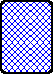
\includegraphics{card_back.pdf}};
	\pic[scale=0.095, transform shape] at (0,0) {head};

}}


\usepackage[hidelinks]{hyperref} % Add hyperlinks to the pdf file. This should usually be the last package loaded before \begin{document}

% Start Document

\begin{document}
% Cover page with title, cover art, description, and author
\center{\setmainfont{Charter}}
{\footnotesize{Version 0.1}}

\setmainfont[Scale=3.075, UprightFont={* 162 Bold}]{Libre Clarendon Normal}
{%\bfseries
\begin{center}
\begin{tabular}{@{}c@{\hspace{0.375ex}}l@{}c@{\hspace{0.425ex}}l@{}}
\Huge{H} & \Huge{\textcolor{red}{E}} & \Huge{A} & \Huge{\textcolor{red}{D}} \\[0.5ex]
\Huge{\textcolor{red}{T}} & \Huge{R} & \Huge{\textcolor{red}{I}} & \Huge{P}
\end{tabular}
\end{center}
}

\vfill

\setmainfont[Scale=1.5]{Charter}
\begin{center}
\LARGE
Headmaster's\phantom{y}Guide
\end{center}

\vfill

\begin{figure}[h]
\centering
	\begin{tikzpicture}
	\node (A) at (0,0) {
\includegraphics[scale=0.06]{head_outline.png}};
	\node (B) at (1.1,0.95) {\fontsize{60}{72}{\hearts}};
	\node (B) at (-1.9,0.95) {\fontsize{60}{72}{\diamonds}};
	\node (B) at (-0.475,2.6) {\fontsize{60}{72}{\spades}};
	\node (B) at (-0.475,-0.4) {\fontsize{60}{72}{\clubs}};
	\end{tikzpicture}
\end{figure}

\vfill

\setmainfont[Scale=1.5]{Charter}
\begin{center}
\LARGE
Michael\phantom{y}Purcell
\end{center}

\newpage

\setmainfont{Charter}
\raggedright
\section{Overview}

\newpage

\section{Setting Cards}
Test

\subsection{Locations}
Each challenge that Bobby faces can occur at one of these locations:
\begin{cardlist}
  \item[\redtwo\diamonds:] Bobby's House
  \item[\redthree\diamonds:] School Bus
  \item[\redfour\diamonds:] Classroom
  \item[\redfive\diamonds:] Cafeteria
  \item[\redsix\diamonds:] Principal's Office
  \item[\redseven\diamonds:] School Hallway
  \item[\redeight\diamonds:] Library
  \item[\rednine\diamonds:] Auditorium
  \item[\redten\diamonds:] Locker Room
\end{cardlist}

\subsection{Non-player Characters}
The challenges that Bobby faces usually involve other people as well.
\begin{cardlist}
  \item[\redjack\diamonds:] Bully
  \item[\redqueen\diamonds:] Crush
  \item[\redking\diamonds:] Friend
\medskip
  \item[\queen\clubs:] Neighbour
  \item[\king\clubs:] Stranger
\medskip
  \item[\redjack\hearts:] Sibling
  \item[\redking\hearts:] Parent
\medskip
  \item[\jack\spades:] Principal
  \item[\queen\spades:] Teacher
\end{cardlist}

\newpage

\section{Conclusion}
test

\vfill

\section{Acknowledgements}
The following people made significant contributions throughout the design process:
\vspace{-1.75ex}
\begin{multicols}{2}
\begin{itemize}[itemsep=0pt, topsep=0pt, partopsep=0pt]
  \item Dannielle Harden
  \item Andrew Hellyer
  \item David McKenzie
  \item Paul Murray
  \item Kira Purcell
  \item Luke Purcell
\end{itemize}
\end{multicols}

\subsection{Design Tools}
The following tools were used to create this leaflet:
\begin{description}[labelindent = 0.25cm, itemsep=0pt, leftmargin=0.25cm]
	\item[Typesetting\normalfont{:}] XeLaTeX.
	\item[Diagrams\normalfont{:}] TikZ, GIMP.
	\item[Fonts\normalfont{:}] Libre Clarendon, Charter, Card~Characters.
\end{description}

\medskip

\textbf{Contact}: \href{mailto:head.trip.card.game@gmail.com}{head.trip.card.game@gmail.com}

\smallskip

\begin{tabular}{@{}m{\textwidth-\widthof{\Huge{\doclicenseIcon}}}@{}m{\widthof{\Huge{\doclicenseIcon}}}@{}}
\footnotesize{This work is licensed under a Creative Commons\newline ``Attribute 4.0 International'' license.} & \Huge{\doclicenseIcon} \\
\end{tabular}
\end{document}